\documentclass{article}
    
    \usepackage{hyperref}
    \usepackage{blkarray} % customed arrays
    \usepackage{amsmath} % matrix equations
    \usepackage{graphicx} % import images
    \usepackage{float} % floating imgs
    \usepackage{subcaption} % several figures on one line
    \usepackage{listings} %source code listing
    \lstset{
        basicstyle=\ttfamily\tiny
    }
    \graphicspath{ {ressources/} }
    
    \title{High Performance Technical Computing}
    \author{Augustin Reille}
    \date{2 November 2017}
    
    \begin{document}
        % Title
        \maketitle
    
        % Abstract
        \begin{abstract}
            A one-space dimensional problem is considered, to examine the application
            of distributed memory parallel programming techniques for the numerical 
            solution of the heat conduction equation.
            % The Dufort-Frankel, Richardson, Laasonen and Crank-Nicolson schemes are implemented,
            % considered, and compared to the analytical solution of the one-space problem.
            % The effect of the time step is investigated for the Laasonen scheme.
            % \\ An object oriented designed C++ code is implemented to point out results.
        \end{abstract}
    
        % Table of contents
        \newpage
        \tableofcontents
    
        % List of figures
        \newpage
        \listoffigures
    
        % List of tables
        \listoftables
    
        % List of listings
        \lstlistoflistings
    
        % List of abbreviations / Nomenclature
        \section*{Nomenclature}
            $T_i^n$ . . . Temperature at space $i$ and time $n$\\
            $D$ . . . . Diffusivity of the wall\\
            $L$ . . . . Total length of the wall\\
            $T$ . . . . Total time of the study\\
            $\Delta x$ . . . Space step\\
            $\Delta t$ . . . Time step\\
            $\delta x$ . . . . partial derivative according to space\\
            $\delta t$ . . . . partial derivative according to time\\
            $n_{space}$. . .  number of iterations over space\\
            $n_{pes}$. . . . number of processors\\
        % Introduction
        \newpage
        \section{Introduction}
    
        % --------- TODO --------- 
        A PDE (Partial Differential Equation) is an equation which includes derivatives of an unknown function, with at least 2 variables.
        PDEs can describe the behavior of lot of engineering phenomena \cite{pde}, that's why it is important to 
        known how to resolve them computationally. One way to resolve PDEs is to discretize the problem into
        a mesh. Applying finites differences on some points of the mesh, we can find a function
        which is more or less the same than the unknown function described by the PDE.
        \\
        To find the unknown function, applying differences on a mesh work differently according to the difference chosen, 
        but also according to the chosen mesh. For a one-dimensional problem, time steps and space steps can impact the accuracy
        of the result found. Also, the chosen differences affect the result. A discretisation scheme is the way we choose to apply
        finites differences.
        \\
        In this study we are going to see how the accuracy of known schemes are evolving for a one-dimensional problem, and how the 
        meshing impact the accuracy of those schemes.
        
        
    
    
        % Methods / Procedures
        \newpage
        \section{Methods}
            Our study results are to be stored in some matrixes, each matrix corresponding to one method.\\
            Several schemes are used :
            \begin{itemize}
                \item{FTCS simple explicit (forward time, central space, explicit)}
                \item{Laasonen simple implicit (forward time, central space, implicit)}
                \item{Crank-Nicholson (Trapezoidal)}
            \end{itemize}
            For all of the used schemes, the initialization of the result matrix is run the same way.
            First the study grid must be chosen. The initials conditions are:
            \begin{itemize}
                \item{$T_{int}$ of 100$^{\circ}$F}
                \item{$T_{sur}$ of 300$^{\circ}$F}
                \item{$D = 0.1 ft^{2}/hr$}
            \end{itemize}
            For each methods two sets of step size are to be used:
            \begin{enumerate}
                \item{$\Delta x = 0.5$ and $\Delta t = 0.1$} 
                \item{$\Delta x = 0.005$ and $\Delta t = 0.001$} 
            \end{enumerate}
            so that the result matrix could be initialized.
            We set:
            \begin{equation}
                n_{space} = \frac{L}{\Delta x} + 1
            \end{equation}
            \begin{equation}
                n_{time} = \frac{T}{\Delta t}
            \end{equation}
            $n_{space}$ is the number of iterations over the grid, according to the coordinate $x$. \\
            $n_{time}$ is the number of iterations over the grid, according to the time $t$. \\
            
            \[
                \begin{blockarray}{cccccc}
                i=0 & i=1 & \cdots & n_{space}-1 & n_{space} \\
                \begin{block}{(ccccc)c}
                  T_{ext} & T_{int} & \cdots & T_{int} & T_{ext} & j=0 \\
                  T_{ext} & 0 & \cdots & 0 & T_{ext} & j=1 \\
                  \vdots & \vdots & \ddots & \vdots & \vdots & \vdots \\
                  T_{ext} & 0 & \cdots & 0 & T_{ext} & n_{time} \\
                \end{block}
                \end{blockarray}
            \]
            This is how the matrix is initialized, according to initial conditions.

            % For most of the used schemes, we need two previous time steps to calculate the current step.
            % An order one scheme (FTCS) is used to find the second line of the matrix:
            % \begin{equation}
            %     T_{i,1} = \frac{\alpha}{2} (T_{i+1,0} + T_{i-1,0}) + (1-\alpha)T_{i,0}
            % \end{equation}
            % with $$\alpha = 2\frac{D\delta t}{\delta x^{2}}$$
            % So we have:
            % \[
            %     \begin{blockarray}{cccccc}
            %     i = 0 & i = 1 & \cdots & n_{space}-1 & n_{space} \\
            %     \begin{block}{(ccccc)c}
            %       T_{ext} & T_{int} & \cdots & T_{int} & T_{ext} & j=0 \\
            %       T_{ext} & T_{i,1} & \cdots & T_{i,1} & T_{ext} & j=1 \\
            %       \vdots & \vdots & \ddots & \vdots & \vdots & \vdots \\
            %       T_{ext} & 0 & \cdots & 0 & T_{ext} & n_{time} \\
            %     \end{block}
            %     \end{blockarray}
            % \]
            % With this trick our matrix is ready to be used and filled up with every scheme.
    
            \subsection{FTCS simple explicit}
                
            In order to perform the parallelization, we assume that the number of 
            space steps can be divided by the number of processors. The number of
            space steps divided by the number of processors defines the new space
            step for each processor:
            \begin{equation}
                n'_{space} = \frac{n_{space}}{n_{pes}}
            \end{equation}
            The stencil for FTCS explicit scheme is the following:
            \begin{figure}[H]
                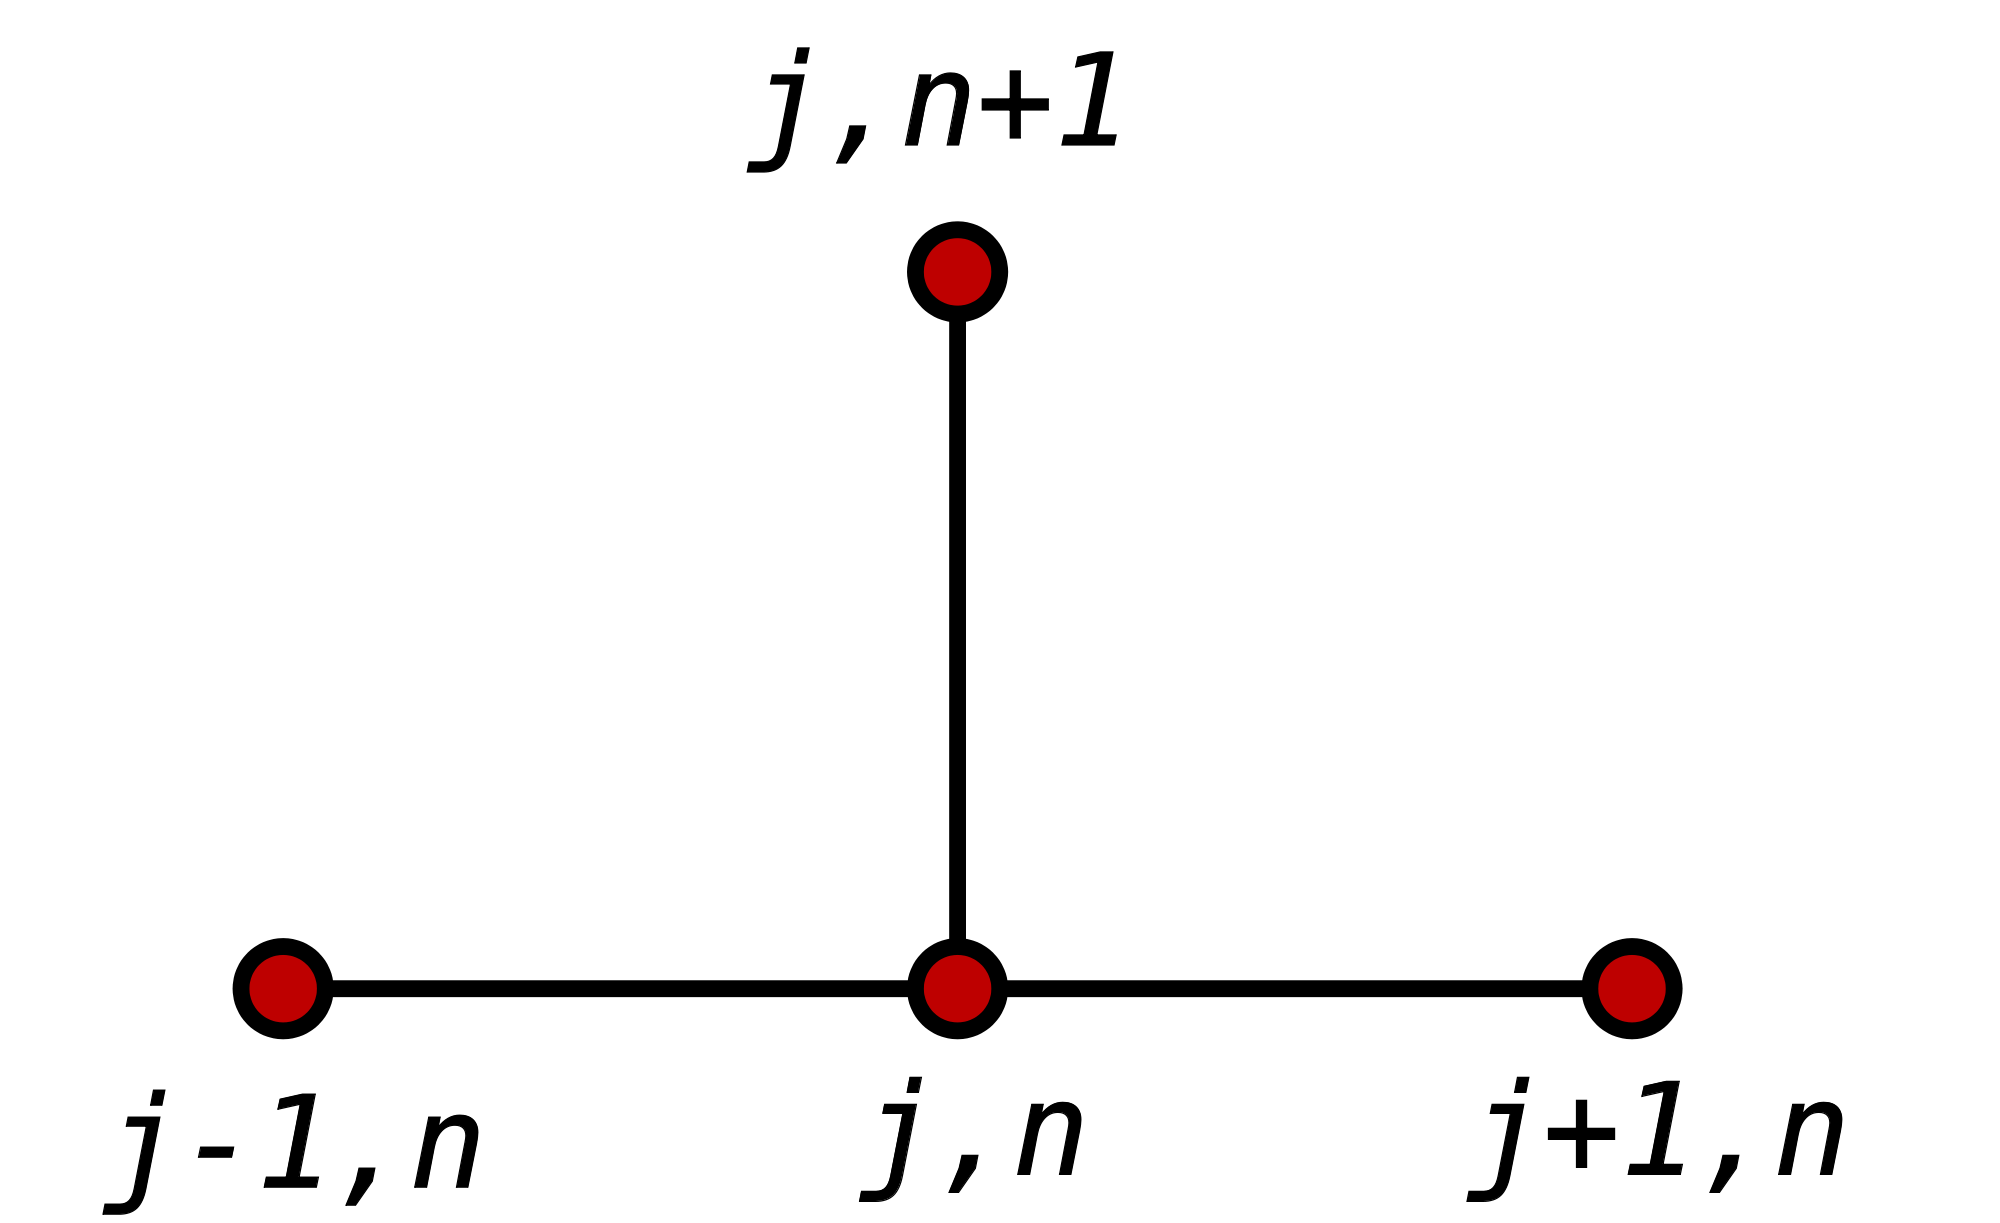
\includegraphics[width=4cm]{stencil_explicit.png}
                \centering
                \caption{Stencil for FTCS explicit scheme}
            \end{figure}

            That means that to calculate a temperature for a time step and a space
            step, we need some previous values in time : the value in space, 
            which we can access easily, and the previous and next values in space.
            That was the main problem for parallelizing this problem. The way we managed
            it is the following.\\
            For each processor, a vector of size $[n'_{space} + 2]$ is created. The size is incremented
            by 2 because each vector will contain 2 "ghost" values (will be explained later).\\
            The first vector will be our boundary values vector, so we fill this vector
            with $T_{int}$.\\
            For the first and last processor respectively, the first and last value of the vector are
            replaced by $T_{ext}$.\\
            For example, for $n_{space} = 12$ and $n_{pes} = 4$, at $t=0h$ we have :
            \begin{figure}[H]
                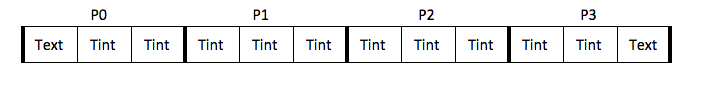
\includegraphics[width=\textwidth]{separation.png}
                \caption{Separation at t=0h}
            \end{figure}

            At each time step, each processor perform 4 MPI actions:
            \begin{itemize}
                \item{it sends its first value to the previous processor (MPI\_Send()) }
                \item{it receives the first value of the next processor (MPI\_Receive())}
                \item{it sends its last value to the next processor (MPI\_Send())}
                \item{it receives the first value of the previous processor (MPI\_Receive())}
            \end{itemize}
            N-B : In the previous explanation, ghost values are not considered : they are only used
            to store the values received from neighbour processors.\\
            In Figure 3, we can see which values are exchanged at the boundaries, in order to
            calculate the next boundary value. This pattern is due to the stencil : to continue
            with the example of the Figure 3, in order to calculate the value of $h[1]$ at time step
            $t+\Delta{t}$, the processor needs the $h[0]$ value, which comes from the previous processor.
            \begin{figure}[H]
                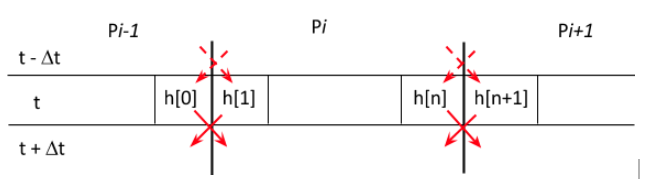
\includegraphics[width=\textwidth]{parallel_explicit.png}
                \caption{Exchanges between processors at each time step}
            \end{figure}

            Calculated values are gathered (MPI\_Gather()) in the final result matrix, which is stored in root processor.

    
            \subsection{Implicit schemes}
    
                    For both implicit schemes, the vector solution is given by a matrix equation. A $LU$
                    factorization is used once, before a for-loop, to resolve the system for each space step.
    
                    \subsubsection{Laasonen}
    
                    We have :
                    \begin{equation}
                        \frac{T_{j}^{n+1} - T_{j}^n}{\Delta t} = D \frac{T_{j+1}^{n+1}- 2T_{j}^{n+1} + T_{j-1}^{n+1}}{\Delta x^2}
                    \end{equation}
    
                    Written in a matrical way, the solution at space step $n+1$ is given by :
                    \begin{equation}
                        \label{eq:laas}
                        \begin{bmatrix}
                            1+2C   & -C     & 0      & \cdots & 0 \\
                            -C     & 1+2C   & -C     & \ddots & \vdots \\
                            0      & -C     & \ddots & \ddots & 0 \\
                            \vdots & \ddots & \ddots & 1+2C   & -C\\
                            0      & \cdots & 0      & -C     & 1+2C
                        \end{bmatrix}
                        \begin{bmatrix}
                            T_{1} \\
                            T_{2} \\
                            \vdots \\
                            T_{i} \\
                            \vdots \\
                            T_{ntime}
                        \end{bmatrix}_{n+1}
                        =
                        \begin{bmatrix}
                            T_{1} + CT_{0}\\
                            T_{2} \\
                            \vdots \\
                            T_{i} \\
                            \vdots \\
                            T_{ntime} + CT_{f}
                        \end{bmatrix}_{n}
                    \end{equation}
                    with $$C = \frac{D\Delta t}{\Delta x ^2}  $$ 
                    The first vector at space $n$ is our boundaries conditions vector, so it is known.
                    In this scheme we must be aware that the right-term vector is actually bigger than
                    the other, of 2 values, which corresponds to the exterior temperatures, which stays
                    the same all the time.\\
                    We apply the $LU$ solve algorithm for each space step, at the reduced vector, and add the $n+1$ vector to our 
                    result matrix. The new right term vector is the one found with the $LU$ solve algorithm.
     
                    \subsubsection{Crank-Nicholson}
                        We have :
                        \begin{equation}
                            \frac{T_{j}^{n+1} - T_{j}^n}{\Delta t} = D\frac{1}{2} (\frac{T_{j+1}^{n+1}- 2T_{j}^{n+1} + T_{j-1}^{n+1}}{\Delta x^2}+\frac{T_{j+1}^{n}- 2T_{j}^{n} + T_{j-1}^{n}}{\Delta x^2})
                        \end{equation}
                        Written in a matrical way, the solution at space step $n+1$ is given by :
                        \begin{equation}
                            \begin{bmatrix}
                                1+C    & -C/2   & 0     & \cdots & 0 \\
                                -C/2   & 1+C    & -C/2   & \ddots & \vdots \\
                                0      & -C/2   & \ddots & \ddots & 0 \\
                                \vdots & \ddots & \ddots & 1+C   & -C/2\\
                                0      & \cdots & 0      & -C/2   & 1+C
                            \end{bmatrix}
                            \begin{bmatrix}
                                T_{1} \\
                                T_{2} \\
                                \vdots \\
                                T_{i} \\
                                \vdots \\
                                T_{ntime}
                            \end{bmatrix}_{n+1}
                            \label{eq:crank}
                        \end{equation}
                        \[
                            =
                            \begin{bmatrix}
                                1-C    &C/2    & 0      & \cdots & 0 \\
                                C/2     & 1-C   & C/2     & \ddots & \vdots \\
                                0      & C/2     & \ddots & \ddots & 0 \\
                                \vdots & \ddots & \ddots & 1-C   & C/2\\
                                0      & \cdots & 0      & C/2     & 1-C
                            \end{bmatrix}
                            \begin{bmatrix}
                                T_{1} + CT_{0}\\
                                T_{2} \\
                                \vdots \\
                                T_{i} \\
                                \vdots \\
                                T_{ntime} + CT_{f}
                            \end{bmatrix}_{n}
                        \]
                        with $$C = \frac{D\Delta t}{\Delta x ^2}  $$ 
                        The method is the same as Laasonen scheme, except that the left term vector found with the $LU$ solve
                        algorithm is multiplied by the right term matrix before the next space step.
    
                \subsection{Analytical solution}
                    The analytical solution of the problem considered will be used to compare our results and to calculate
                the errors. The result of the analytical solution for a time $t$ and a position $x$ is given by : 
                \begin{equation}
                    \label{eq:analytical}
                    T = T_{ext}+2(T_{int}-T_{ext})\sum_{m=1}^{m=\infty} e^{-D(m\pi / L)^{2}t} \frac{1-(-1)^m}{m\pi} sin(\frac{m\pi x}{L})
                \end{equation}
    
    
                \subsection{Object Oriented Design}
    
                The object oriented classes for the C++ code are designed the following way :\\
                \begin{figure}[H]
                    % \includegraphics[width=\textwidth]{UML.png}
                    \caption{UML Diagram of the C++ object oriented code}
                \end{figure}
                There is a main base class called PDESolve, which initializes all the variables, and two functions :
                \begin{itemize}
                    \item{get\_res() : returns the results Matrix}
                    \item{solve() : virtual function which will be overwritten in subclasses}
                \end{itemize}
                There is two subclasses of PDESolve : PDEExplicit and PDEImplicit. Each one has a solve() function, and a virtual advance function,
                which corresponds at the way the space and time steps are incrementded.
                The PDEImplicit class also initializes all the matrixes and functions needed for the LU factorization and solve.
                Each subsubclass, which corresponds to each method, has its own particular advance method.
        % Results
        \newpage
        \section{Results}
            \subsection{Schemes study}
                Note that results from Richardson scheme are not displayed on the following plots, due to its unstability \cite{rich}: 
            the incorrect values polluted our charts.
            \begin{figure}[H]
                % \includegraphics[width=\textwidth]{t01.png}
                \caption{Results with differents schemes at t = 0,1h}
            \end{figure}
            We can see that except for the Richardson scheme, the results are quite the same. The errors had been calculated 
            to evaluate the accuracy of each method.
            \begin{table}[H]
                \centering
                \caption{Errors for different schemes at t = 0,1h}
                \begin{tabular}{|c|c|c|c|l}
                \cline{1-4}
                Errors & Dufort-Frankel & Laasonen & Crank-Nicholson &  \\ \cline{1-4}
                1-norm & 0,56\%         & 1,72\%   & 1,26\%          &  \\ \cline{1-4}
                \end{tabular}
            \end{table}
            We observe that Dufort-Frankel method is the most accurate, 
            followed by the Crank-Nicholson method then by the Laasonen method. Let see the evolution of the error
            while we advance in time. (see appendix for plots)
            
            \begin{table}[H]
                \centering
                \caption{Errors for different schemes at different times}
                \begin{tabular}{|c|c|c|c|}
                \hline
                Errors & Dufort frankel & Laasonen & Crank-Nicholson \\ \hline
                t=0,2h & 0,37\%         & 1,05\%   & 0,80\%          \\ \hline
                t=0,3h & 0,27\%         & 0,77\%   & 0,60\%          \\ \hline
                t=0,4h & 0,22\%         & 0,64\%   & 0,49\%          \\ \hline
                t=0,5h & 0,18\%         & 0,55\%   & 0,42\%          \\ \hline
                \end{tabular}
            \end{table}
    
            We observe that the error is globally decreasing as time increase. The most accurate method appears to 
            be the Dufort-Frankel method, then the Crank-Nicholson method, then the Laasonen method.
    
            \subsection{Laasonen method : effect of the step time}
            \begin{figure}[H]
                % \includegraphics[width=\textwidth]{analytical.png}
                \caption{Analytical results at different times}
            \end{figure}
            \begin{figure}[H]
                % \includegraphics[width=\textwidth]{las-1.png}
                \caption{Laasonen scheme with $\Delta t$ = 0,01}
            \end{figure}
            
            We can see that the shape of the results is more accurate as $\Delta t$ is little.
            It may be assumed that increasing $\Delta t$ gives less accurate results.
            Let's calculate the error between these values and the analytical values. (See appendix for plots)
    
            \begin{table}[H]
                \centering
                \caption{Laasonen - effect of time step increasing }
                \label{table:laas}
                \begin{tabular}{|l|l|l|l|l|l|}
                    \hline
                    Errors    & t = 0,1h & t = 0,2h  & t = 0,3h  & t = 0,4h & t = 0,5h \\ \hline
                    $\Delta$t=0,01  & 1,72\%   & 1,05\%  & 2,83\%  & 0,64\% & 0,55\% \\ \hline
                    $\Delta$t=0,025 & 4,53\%   & 2,76\%  & 0,81\%  & 1,69\% & 1,45\% \\ \hline
                    $\Delta$t=0,05  & 9,75\%   & 5,84\%  & 4,95\%  & 3,50\% & 2,98\% \\ \hline
                    $\Delta$t=0,1   & 53,96\%  & 12,80\% & 16,30\% & 7,35\% & 6,19\% \\ \hline
                \end{tabular}
            \end{table}
    
            We observe that as time grows, the error decrease. Also, as time step grows, the error is increasing.
            Previous asumption is correct, according to the error calculation.
        % Discussion
        \newpage
        \section{Discussion}
            \subsection{Analytical solution}
                First thing that should be considered is that the analytical solution should not be
                considered as the perfect exact solution, because of several factors.
                \\
                First, the analytical solution is calculated by the computer, so there may be some numerical error.
                \\
                Secondly, we have to consider the calculation of the sum inside equation \eqref{eq:analytical}.
                Indeed, as $m$ should be infinite, the biggest it is is the best. However, as I choose to calculate
                all the results for each time step, increasing $m$ also increase run time. I choosed a compromise
                where values of the analytical solution at $t=0$ were as correct as possible, with an $m$ not too big,
                to reduce run time.
                \\
                \\
                Though, it may have been a good idea to calculate the analytical solutions only at studied times : 
                it would have reduced the memory usage, and we could have afforded to increase the value of $m$.
                This would have given us better values for our errors calculation.
    
            \subsection{Computational study}
                \subsubsection{LU factorization and solving}
                    LU factorization and solving is used in the C++ code. However, Thomas algorithm could have been used for several 
                    reasons.
                    \\
                    First, our matrix is tridiagonal, which is a condition to use Thomas algorithm.
                    \\
                    Secondly, Thomas algorithm has a smaller complexity ($O(n)$) than LU solving ($O(n^3)$), it is also faster.
                    \\
                    This way, we would have reduced the total complexity of our code and the computational time.
                \subsubsection{Vectors}
                    Another way to reduce the complexity of our code and the used memory would have been to use vectors instead
                    of matrixes in equations \eqref{eq:laas} and \eqref{eq:crank}. Indeed, for the implicit methods, most of our matrixes are filled up with zeros, and every line is
                    the same, only the position of the values change. We could have used only one vector of size 3 instead of a quite big matrix.
                    It is quite all right for this study because we are working with only two dimensions, and with a quite reduced space.
                    By moving in a more complex problem, delays would have appeared.
            \subsection{Schemes study}
                \subsubsection{Richardson scheme}
                    We saw that Richardson scheme was unstable \cite{rich}. Also, when we change the $T_{i}^n$ term
                    in \eqref{eq:rich} by the average $\frac{(T_i^{n+1}+T_i^{n-1})}{2}$, we obtain the following :
                    \begin{equation}
                        T_i^{n+1} = T_i^{n-1} + \frac{2D\delta t}{\delta x^2}[T_{i+1}^n - (T_i^{n+1}+T_i^{n-1}) + T_{i-1}^n]
                    \end{equation}
                    Which is equivalent as \eqref{eq:df}, the Dufort-Frankel scheme, which is a stable scheme \cite{df}.
                    \\
                    So we can see that by replacing the $T_{i}^n$ term in an unstable scheme by its average in time, we obtain 
                    a stable scheme. This is a good thing to know as majority of explicit schemes are unstable. However, they are
                    easy to test, so that we can easily find some way to make them stable if they are not.
                \subsubsection{Dufort-Frankel versus other schemes}
                    It appears that Dufort-Frankel scheme is the most accurate of the studied schemes. One explanation to those
                    results is that with this method, accurate solutions are obtained if $\Delta t << \Delta x$ \cite{df}, which
                    is our case.
                    The two other schemes, Laasonen and Crank Nicholson seem to have the same accuracy.
                    \\
                    Crank Nicholson scheme needs a low $D$ coefficient for numerical accuracy \cite{crank}, which is our case. That's why 
                    we have a quite good accuracy (less than $1\%$) in our results.
                
            \subsection{Laasonnen method : effect of the step time}
                As we see on Table \ref{table:laas}, for a fixed $\Delta t$, the error tends to decrease as time grows. However,
                for a fixed time, we can see that increasing the time step make the error bigger. We can assume that we need a
                quite small time step to have good results with this scheme. This can be explained by the fact that
                Laasonen has a good error response, however it has the disadvantage of a poor accuracy \cite{laas}.
        % Future work
        \newpage
        \section{Future work}
            Our future work would be based on three major axes : memory, runtime and interface optimization.
            It would be interesting to take a smaller time step, and to try to test our program
            with a parallel programming model, and run it on an HPC, as we have the opportunity 
            to work on one here at Cranfield University.
            \subsection{Memory optimization}
                As said previously, memory use could be improved by at least two manners :
                \begin{itemize}
                    \item{Calculate only the values which will be used in the study}
                    \item{For implicit schemes, replace the tridiagonal matrix by one vector}
                \end{itemize}
            \subsection{Runtime optimization}
                As said before, since we have a small study scale, it is not crucial to have a good
                runtime optimization. However, we still could optimize the runtime, particularly
                by using Thomas algorithm instead of LU algorithm.
            \subsection{Interface optimization}
                We also could improve the way the results are printed : here we write them brutally
                in our main function, or in a CSV file, which is used in a spreadsheet application
                in order to print graphics.
                \\
                Maybe a little interface more user-friendly could be developped, using QT or something
                else, with the possibility for the user to input data, initial conditions, the chosen
                scheme, and with the printing of graphics and errors value.
    
        % Conclusion
        \newpage
        \section{Conclusion}
            For a one dimensional problem, PDE can be resolved using discretisation schemes. In this study
            we saw that several schemes can fit for this kind of problem. However, some schemes appears to
            be more accurate.\\
            The accuracy of all the schemes seems to be impacted by common causes:
            \begin{itemize}
                \item{Error grows as time step grows : the smallest time step must be used, while complying with
                the computational ressources that are at our disposal (indeed, numerical computational error could appear)}
                \item{Error tends to decrease as the time study grows}
            \end{itemize}
            
            However, there is some factors which gives each scheme particular accuracy.\\
            \\
            Resolving PDE with computational methods also introduce numerical errors, due to the computers way
            of calculating. Depending on the power of the computer we use, we must try to be as precise as possible
            by setting a study mesh with a grid as small as possible. Some other study with different computational ressource
            could teach us about the effect of a very small grid, i.e. the effect of a lot more calculations.
            
        % Aknowledgments
        % \newpage
        % \section{Aknowledgments}
    
        % References
        \newpage
        \section{References}
        \begin{thebibliography}{9}
            \bibitem{pde}
            Wazwaz, Abdul-Majid. \textit{Partial differential equations}. CRC Press, 2002.
    
            \bibitem{rich} 
            Markus Schmuck - Numerical Methods for PDEs,
            \\\texttt{http://www.macs.hw.ac.uk/\~ms713/lecture\_9.pdf}.
            \\Last visit date : 18/11/2017
    
            \bibitem{df} 
            A. Salih - Finite Difference Method for Parabolic PDE,
            \\\texttt{https://www.iist.ac.in/sites/default/files/people/parabolic.pdf}.
            \\Last visit date : 18/11/2017
    
            
            \bibitem{crank} 
            Crank, J. & Nicolson, P. Adv Comput Math (1996) 6: 207. 
            \\\texttt{https://doi.org/10.1007/BF02127704}
    
            \bibitem{laas} 
            D. Britz \& Jorg Strutwolf, \textit{Digital Simulation in Electrochemistry}.
            Springer, 2006
    
            
            % \bibitem{einstein} 
            % Albert Einstein. 
            % \textit{Zur Elektrodynamik bewegter K{\"o}rper}. (German) 
            % [\textit{On the electrodynamics of moving bodies}]. 
            % Annalen der Physik, 322(10):891–921, 1905.
            
        \end{thebibliography}
        % Appendices
        \newpage
        % \section{Appendices}
        %     \subsection{Plots}
        %         \subsubsection{Different schemes study}
        %             \begin{figure}[H]
        %                 \includegraphics[width=\textwidth]{t02.png}
        %                 \caption{Results with differents schemes at t = 0,2h}
        %             \end{figure}
        %             \begin{figure}[H]
        %                 \includegraphics[width=\textwidth]{t03.png}
        %                 \caption{Results with differents schemes at t = 0,3h}
        %             \end{figure}
        %             \begin{figure}[H]
        %                 \includegraphics[width=\textwidth]{t04.png}
        %                 \caption{Results with differents schemes at t = 0,4h}
        %             \end{figure}
        %             \begin{figure}[H]
        %                 \includegraphics[width=\textwidth]{t05.png}
        %                 \caption{Results with differents schemes at t = 0,5h}
        %             \end{figure}
        %         \subsubsection{Laasonen scheme study}
        %             \begin{figure}[H]
        %                 \includegraphics[width=\textwidth]{las-2.png}
        %                 \caption{Laasonen scheme with $\Delta t$ = 0,025}
        %             \end{figure}
        %             \begin{figure}[H]
        %                 \includegraphics[width=\textwidth]{las-3.png}
        %                 \caption{Laasonen scheme with $\Delta t$ = 0,05}
        %             \end{figure}
        %             \subsection{Code sample}
        %             \lstinputlisting[language=C++, caption=PDESolve class header]{../PDESolve.h}
        %             \lstinputlisting[language=C++, caption=PDESolve class code]{../PDESolve.cpp}
        %             \lstinputlisting[language=C++, caption=PDEImplicit class header]{../PDEImplicit.h}
        %             \lstinputlisting[language=C++, caption=PDEImplicit class code]{../PDEImplicit.cpp}
        %             \lstinputlisting[language=C++, caption=PDEExplicit class header]{../PDEExplicit.h}
        %             \lstinputlisting[language=C++, caption=PDEExplicit class code]{../PDEExplicit.cpp}
        %             \lstinputlisting[language=C++, caption=DufortFrankelSolve class header]{../DufortFrankelSolve.h}
        %             \lstinputlisting[language=C++, caption=DufortFrankelSolve class code]{../DufortFrankelSolve.cpp}
        %             \lstinputlisting[language=C++, caption=RichardsonSolve class header]{../RichardsonSolve.h}
        %             \lstinputlisting[language=C++, caption=RichardsonSolve class code]{../RichardsonSolve.cpp}
        %             \lstinputlisting[language=C++, caption=LaasonenSolve class header]{../LaasonenSolve.h}
        %             \lstinputlisting[language=C++, caption=LaasonenSolve class code]{../LaasonenSolve.cpp}
        %             \lstinputlisting[language=C++, caption=CrankNicholsonSolve class header]{../CrankNicholsonSolve.h}
        %             \lstinputlisting[language=C++, caption=CrankNicholsonSolve class code]{../CrankNicholsonSolve.cpp}
        \end{document}